%% This is file `DEMO-TUDaExercise.tex' version 2.09 (2020/03/13),
%% it is part of
%% TUDa-CI -- Corporate Design for TU Darmstadt
%% ----------------------------------------------------------------------------
%%
%%  Copyright (C) 2018--2020 by Marei Peischl <marei@peitex.de>
%%
%% ============================================================================
%% This work may be distributed and/or modified under the
%% conditions of the LaTeX Project Public License, either version 1.3c
%% of this license or (at your option) any later version.
%% The latest version of this license is in
%% http://www.latex-project.org/lppl.txt
%% and version 1.3c or later is part of all distributions of LaTeX
%% version 2008/05/04 or later.
%%
%% This work has the LPPL maintenance status `maintained'.
%%
%% The Current Maintainers of this work are
%%   Marei Peischl <tuda-ci@peitex.de>
%%   Markus Lazanowski <latex@ce.tu-darmstadt.de>
%%
%% The development respository can be found at
%% https://github.com/tudace/tuda_latex_templates
%% Please use the issue tracker for feedback!
%%
%% ============================================================================
%%
% !TeX program = lualatex
%%

\documentclass[
	ngerman,
	]{tudaexercise}

\usepackage[english]{babel}
\usepackage[babel]{csquotes}
\usepackage{listings}
\usepackage{graphicx}
\usepackage{float} 
\usepackage{subfigure}

\usepackage{biblatex}
\bibliography{DEMO-TUDaBibliography}

%Formatierungen für Beispiele in diesem Dokument. Im Allgemeinen nicht notwendig!
\let\file\texttt
\let\code\texttt
\let\pck\textsf
\let\cls\textsf
\let\tbs\textbackslash

\ConfigureHeadline{
	headline={title-name-id}
}

\definecolor{dkgreen}{rgb}{0,0.6,0}
\definecolor{gray}{rgb}{0.5,0.5,0.5}
\definecolor{mauve}{rgb}{0.58,0,0.82}

\lstset{frame=tb,
  language=Python,
  aboveskip=3mm,
  belowskip=3mm,
  showstringspaces=false,
  columns=flexible,
  basicstyle={\small\ttfamily},
  numbers=left,
  backgroundcolor=\color[RGB]{245,245,244},  
  numberstyle=\tiny\color{gray},
  keywordstyle=\color{blue},
  commentstyle=\color{dkgreen},
  stringstyle=\color{mauve},
  breaklines=true,
  breakatwhitespace=true,
  tabsize=3
}

%compatbilitx
\let\unit\relax

\begin{document}

\title[Übung TUDaExercise]{Statistical Machine Learning \\ Exercise 3}
\author{Wenhua Bao, Xinrui Chen}
\term{Sommersemester 2020}


\maketitle
\begin{task}{Linear Regression}

\end{task}

\begin{task}{Linear Classification}

\end{task}

\begin{task}{Principal Component Analysis}

\begin{subtask}
Normalizing can convert the original data into pure,dimensionless values and remove the unit restriction on data, then it is easy to compare and weight indicator among data with different units or scales. After Normalizing the data is easy to handle. One Advantage is that the convergence speed of the model improves. For example, if there is only two features, and the range of component 1is 1000 and the range of component 2 is 5. The speed of iteration is very low during the optimization. But after normalizing the speed will be faster. Another advantage is that the accuracy of the model improves. In the last example, when we need to calculate about the distance, the second feature make much less contribute to the result than the first one.

Code:
\begin{lstlisting}
import numpy as np
import matplotlib.pyplot as plt
# get data
iris = np.loadtxt("./dataSets/iris.txt", delimiter=',')
iris_set = iris[:, 0:4]
iris_label = iris[:, 4]
# Normalizing
iris_norm = (iris_set-np.mean(iris_set, axis=0))/np.std(iris_set, axis=0)
print('mean:', np.mean(iris_norm, axis=0))
print('var:', np.var(iris_norm, axis=0))
\end{lstlisting}

\end{subtask}

\begin{subtask}
We need only two components to in order to explain at least 95\% of the dataset variance. From the picture below, we can know that the cumulative variance of first two components is 95.8010\%.\\

\begin{figure}[H] 
\centering 
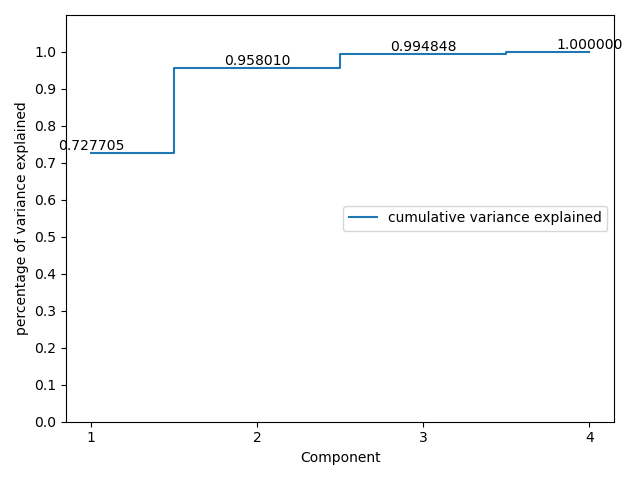
\includegraphics[width=0.7\textwidth]{pic1} 
\caption{cumulative variance explained} 
\label{Fig.main2} 
\end{figure}

Code:
\begin{lstlisting}
#PCA
cov_matrix = np.cov(iris_norm, rowvar=0)
eigenvalues, eigenvectors = np.linalg.eig(cov_matrix)
eigenvalues_sorted = np.sort(eigenvalues)[-1::-1]
total = np.sum(eigenvalues_sorted)
var_explained = np.zeros(4)
for i, item in zip(range(4), eigenvalues_sorted):
    var_explained[i] = item/total
cum_var_explained = np.cumsum(var_explained)
x = ['1','2','3','4']
plt.step(x, cum_var_explained, where='mid', label='cumulative variance explained')
for a, b in zip(x, cum_var_explained):
    plt.text(a, b, '%f' % b, ha='center', va='bottom')
plt.ylim((0, 1.1))
plt.yticks(np.arange(0,1.1,0.1))
plt.xlabel('Component')
plt.ylabel('percentage of variance explained')
plt.legend(loc='center right')
plt.show()
\end{lstlisting}

\end{subtask}

\begin{subtask}
From the picture below, we can know that the data can be clearly distinguished by using 2 components, specially, through component1 the data is distinguished. Two components can explain 95\% of the dataset variance. After PCA we spared two feature, i.e., 50\% data, but the data can be still good distinguished and only 5\% dataset variance is lost.
\begin{figure}[H] 
\centering 
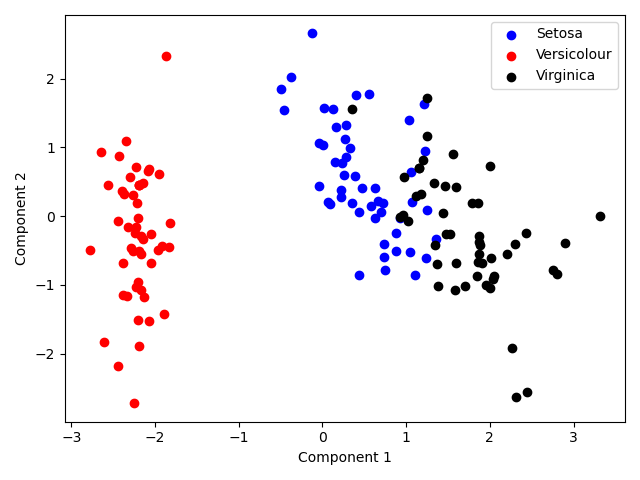
\includegraphics[width=0.7\textwidth]{pic2} 
\caption{ lower dimensional projection} 
\label{Fig.main2} 
\end{figure}

Code:
\begin{lstlisting}
vector_n = eigenvectors[:,0:2]
iris_lowDim = iris_norm@vector_n
name =['Setosa', 'Versicolour', 'Virginica']
print(iris_lowDim.shape)
for lab, col in zip(range(3), ('blue', 'red', 'black')):
     plt.scatter(iris_lowDim[iris_label==lab, 0], iris_lowDim[iris_label==lab, 1], label=name[lab], color=col)
plt.xlabel('Component 1')
plt.ylabel('Component 2')
plt.legend()
plt.show()
\end{lstlisting}

\end{subtask}

\begin{subtask}

\begin{tabular}{|c|c|c|c|c|}
\hline  
N. of components&x1&x2&x3&x4\\
\hline  
1&0.22925036&0.18006108&0.29805579&0.31692192\\
\hline
2&0.11261513&0.19281695&0.13314032&0.12717403\\
\hline
3&0.07919279&0.23615959&0.13302896&0.1257637\\
\hline
4&0.04925365&0.23658978&0.1322316&0.10227491\\
\hline
\end{tabular}
\\
\\Code:
\begin{lstlisting}
# reconstruct
def nrmse(eigvec,n):
    vec_n = eigvec[:, 0:n]
    lowDim = iris_norm @ vec_n
    std = np.std(iris_set, axis=0)
    iris_reconstruct = lowDim@vec_n.T+np.mean(iris_set, axis=0)
    k = np.max(iris_set, axis=0)-np.min(iris_set, axis=0)
    return np.sqrt(np.mean(np.square(iris_reconstruct-iris_set), axis=0))/k
for n in range(4):
    print(nrmse(eigenvectors, n))
\end{lstlisting}
\end{subtask}

\begin{subtask}
1. Explain the difference between PCA and ZCA whitening.\\
~\\
PCA whitening: It ensures the variance of each dimension of the data is 1.\\
ZCA whitening: It ensures that the variance of each dimension of the data is the same. It does a rotation operation on the basis of PCA whitening to make the data after whitening closer to the original data \\
~\\
2. State the equation(s) to compute the ZCA whitening parameters, given the data.\\
~\\
There are m samples, and the feature dimension of each sample is n. We have a sample set feature matrix X of n rows and m columns. And then we calculate Zero-average each row of X.
The covariance matrix of X:
\begin{equation}\Sigma=\frac{1}{m} X X^{T}\end{equation}
Calculate the eigenvalues and corresponding eigenvectors of the covariance matrix:
\begin{equation}\frac{1}{m} X X^{T}=U A U^{T}\end{equation}
Rotate data
\begin{equation}X_{rot}=U^{T} X\end{equation}
Then we get the PCA whitening	
\begin{equation}X_{PCAwhite, i}=\frac{X_{rot, i}}{\sqrt{\lambda_{i}+e}}, e=1.0 e^{-5}\end{equation}
ZCA whitening:
\begin{equation}X_{ZCAwhite, i}=U X_{PCAwhite, i}\end{equation}\\
~\\
3. State the equation(s) to whiten a (new) data example x, given the ZCA parameters. 
 ~\\
4. Compute and report the ZCA whitening parameters for the unnormalized IRIS data (including numerical values!).\\
\begin{lstlisting}
import numpy as np
# get data
iris = np.loadtxt("./dataSets/iris.txt", delimiter=',')
iris_set = iris[:, 0:4]
iris_label = iris[:, 4]


def ZCA_whitening(x):
    avg = np.mean(x, axis=0)
    x = x - avg
    sigma = np.cov(x, rowvar=0)
    u,s,v = np.linalg.svd(sigma)
    xRot = x@u
    xPCAwhite = xRot / np.sqrt(s + 1e-5)
    xZCAwhite = (u@xPCAwhite.T).T
    return xPCAwhite,xZCAwhite


xPCAwhite, xZCAwhite = ZCA_whitening(iris_set)
print(xZCAwhite)
\end{lstlisting}
result:\\

\begin{figure}[H] 
\centering
\subfigure[data1.]{
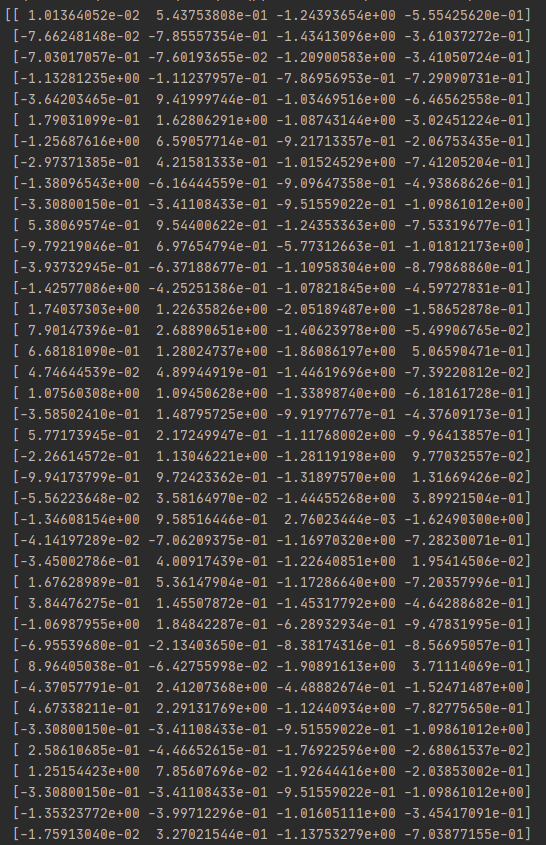
\includegraphics[width=5.5cm]{pic3}
}
\quad
\subfigure[data2.]{
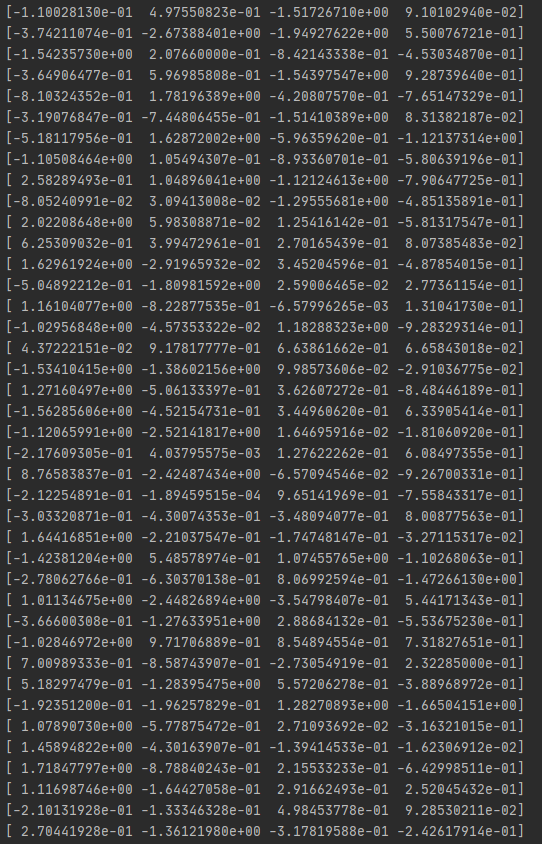
\includegraphics[width=5.5cm]{pic4}
}

\quad
\subfigure[data3.]{
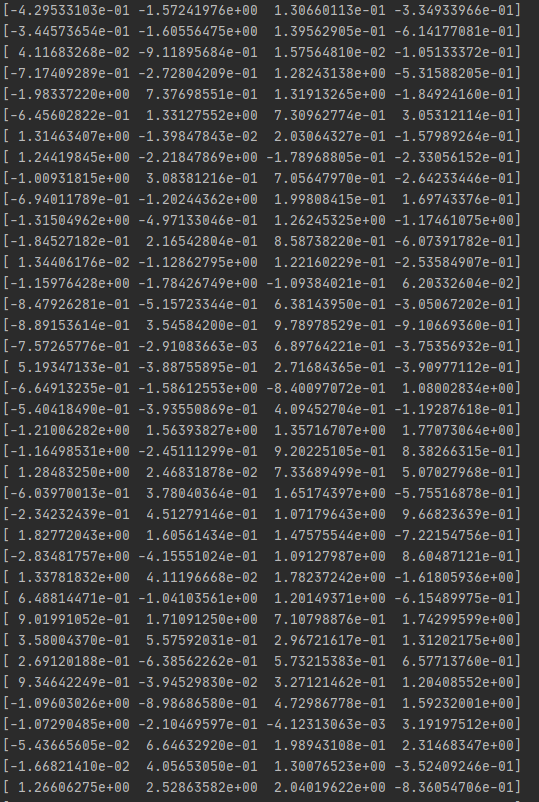
\includegraphics[width=5.5cm]{pic5}
}
\quad
\subfigure[data4.]{
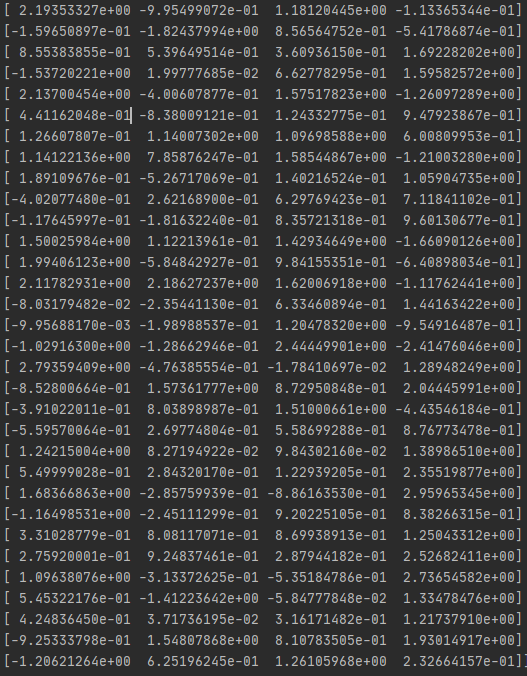
\includegraphics[width=5.5cm]{pic6}
}
\caption{ZCA}
\end{figure}
\end{subtask}

\begin{subtask}

In general, PCA is suitable for linear dimensionality reduction of the data. Kernel Principal Component Analysis enables non-linear dimensionality reduction of data and is used to deal with linear distinguishable data set.The basic idea of KPCA is that for a  input matrix X, by using a nonlinear mapping we map all the samples in X to a high or even infinite dimensional space to making it linearly distinguishable, and then process the data in this high-dimensional space using PCA.\\
\\~
These are the steps for the implementation of the kernel PCA algorithm:\\
1. Choose a kernel mapping $k({\mathbf x}_m,{\mathbf x}_n)$.\\
2. Obtain${\mathbf K}$ based on training data $\{ {\mathbf x}_n, (n=1,\cdots,N)\}$.\\
3. Solve eigenvalue problem of ${\mathbf K}$ to get $\lambda_i$ and ${\mathbf a}_i$.\\
4. For each given data point ${\mathbf x}$, obtain its principal components in the feature space: $(f({\mathbf x})\cdot \phi_i)=\sum_{n=1}^N a_n^{(i)} k({\mathbf x}, {\mathbf x}_n) $\\
5. Do whatever processing (e.g., feature selection, classification) in the feature space.\\
(Reference: http://fourier.eng.hmc.edu/e161/lectures/kernelPCA/node4.html)\\
\\~
Limits: KPCA coats more time than PCA
\end{subtask}

\end{task}

\end{document}
